\chapter{Introduction}
\label{sec:Introduction}

\paragraph{}
-Why is sea ice important, and what are the applications of understanding it at a closer scale?-

\indent In recent decades, understanding the state of sea ice has grown increasingly more important. Sea ice analysis at large scales can provide valuable insight into the trajectory of climate change and at local scale has implications in fields like arctic navigation. Understanding sea-ice thickness in particular, is important for both of these applications.  For example, the thickness of the ice can be analyzed over time to track ice mass in relation to global warning or interpreted locally to predict shipping speed through ice-covered water \cite{sea-ice-properties}.


\indent Due to the harsh nature of the arctic, in-situ studies of arctic ice are infrequent both in time and space. Thus, most analyses depend heavily on remote sensing methods. These methods cumulatively provide magnitudes more data than in-situ measurements can achieve, but differ in modality, methodology and resolution. Synthetic Aperture Radar (SAR) and light detection and ranging (LiDAR) are some such modalities that survey the arctic region. Furthermore, organizations like the the National Aeronautics and Space Administration (NASA) and European Space Agency (ESA) freely provide this information through their constellation of satellites.

% Crop the image to better fit the page. Also include an image that contrasts this availability with the availability of any other remote sensed method.
\begin{figure}[htb]
	\centering
	\subfigure{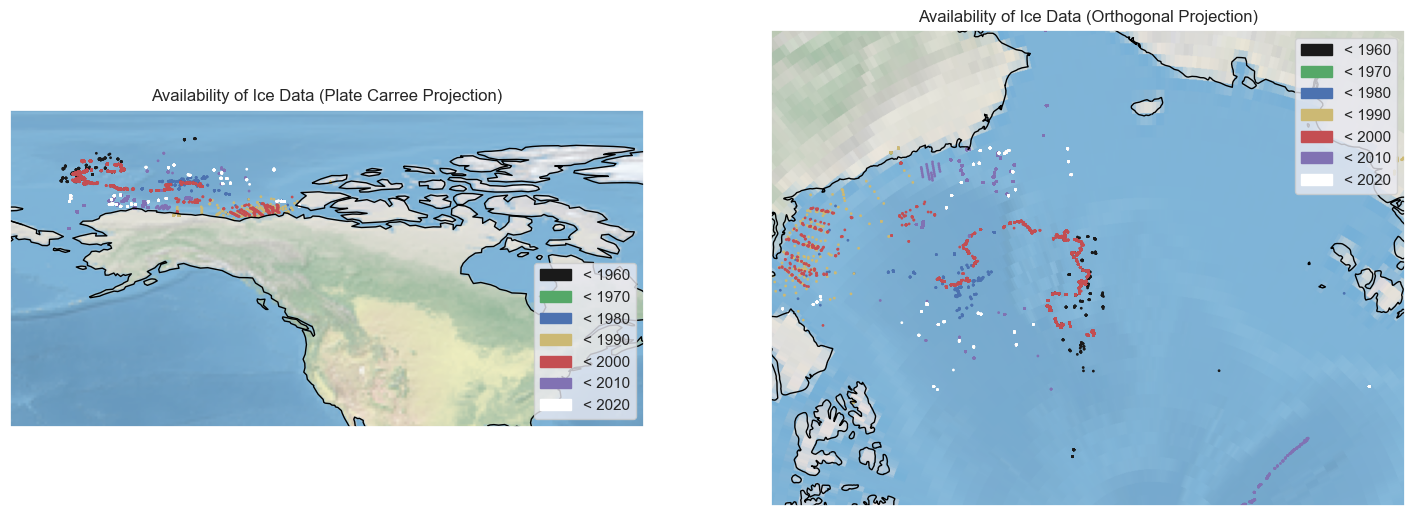
\includegraphics[width=0.8\textwidth]{../research-resources/in-situ/Plotted-Tracks.png}} 
	\caption{Historic In-Situ Data Availability in the Beaufort Sea Region}
	\label{fig:foobar}
\end{figure}

Each of these remote sensing methods have their individual strengths and limitations. ICESat-2 (IS-2), a NASA LiDAR satellite, works by emitting individual photons and timing their returns.
Praised for its precision, its readings are statistically corrected to adjust for ambient light, cloud occlusion (atmospheric scattering), snow and ice scattering, and the physical problem of first-photon bias \cite{ICESat-2-ATL10-Product}.
IS-2's statistical robustness offers valuable local observation with less than 5 meters of total geolocation error (mean \(+ 1\sigma\)) \cite{ICESat-2-Horizontal-Accuracy}.

In contrast to IS-2's highly accurate and local measurements, SAR imaging offers significantly more expansive data with a loss in local precision. SAR images Earth's surface by emitting radio waves and then reconstructing the surface composition based upon the return signal. The physical difference between photons and radio waves means that LiDAR's limitations with occlusion are actually imperceptible to SAR satellites. Radio waves permeate clouds and snow, and the reconstructed image is independent of light \cite{SAR-Info}. These weather independent properties make SAR an excellent modality to monitor sea ice especially during winter seasons, with satellites like Sentinel-2 (SN-2) from NASA offering 290 kilometer swaths of imaging, at resolutions ranging between 10 and 60 meters \cite{Sentinel-2-Availability}. It's important to note that despite its extensiveness, SAR is more sensitive to physical factors like surface roughness, slant, and type, and also suffers from speckle noise \cite{SAR-Info}. 

\indent Given the availability of remote sensed data and their different observed properties, there is much to be learned about the state of the sea ice by corroborating these data sources with each other. Uniquely, the corroboration of a SAR image with precise LiDAR measurements suggests the possibility of developing a convolutional neural network (CNN) to accurately predict sea ice thickness using expansive SAR imaging. Doing so successfully would effectively map IS-2's precision onto the weather agnostic, extensive imaging gathered by SAR satellites, thus allowing for local scale analysis of sea ice across large regions.

\begin{figure}
	\hfill\begin{minipage}{.5\textwidth}\centering
	 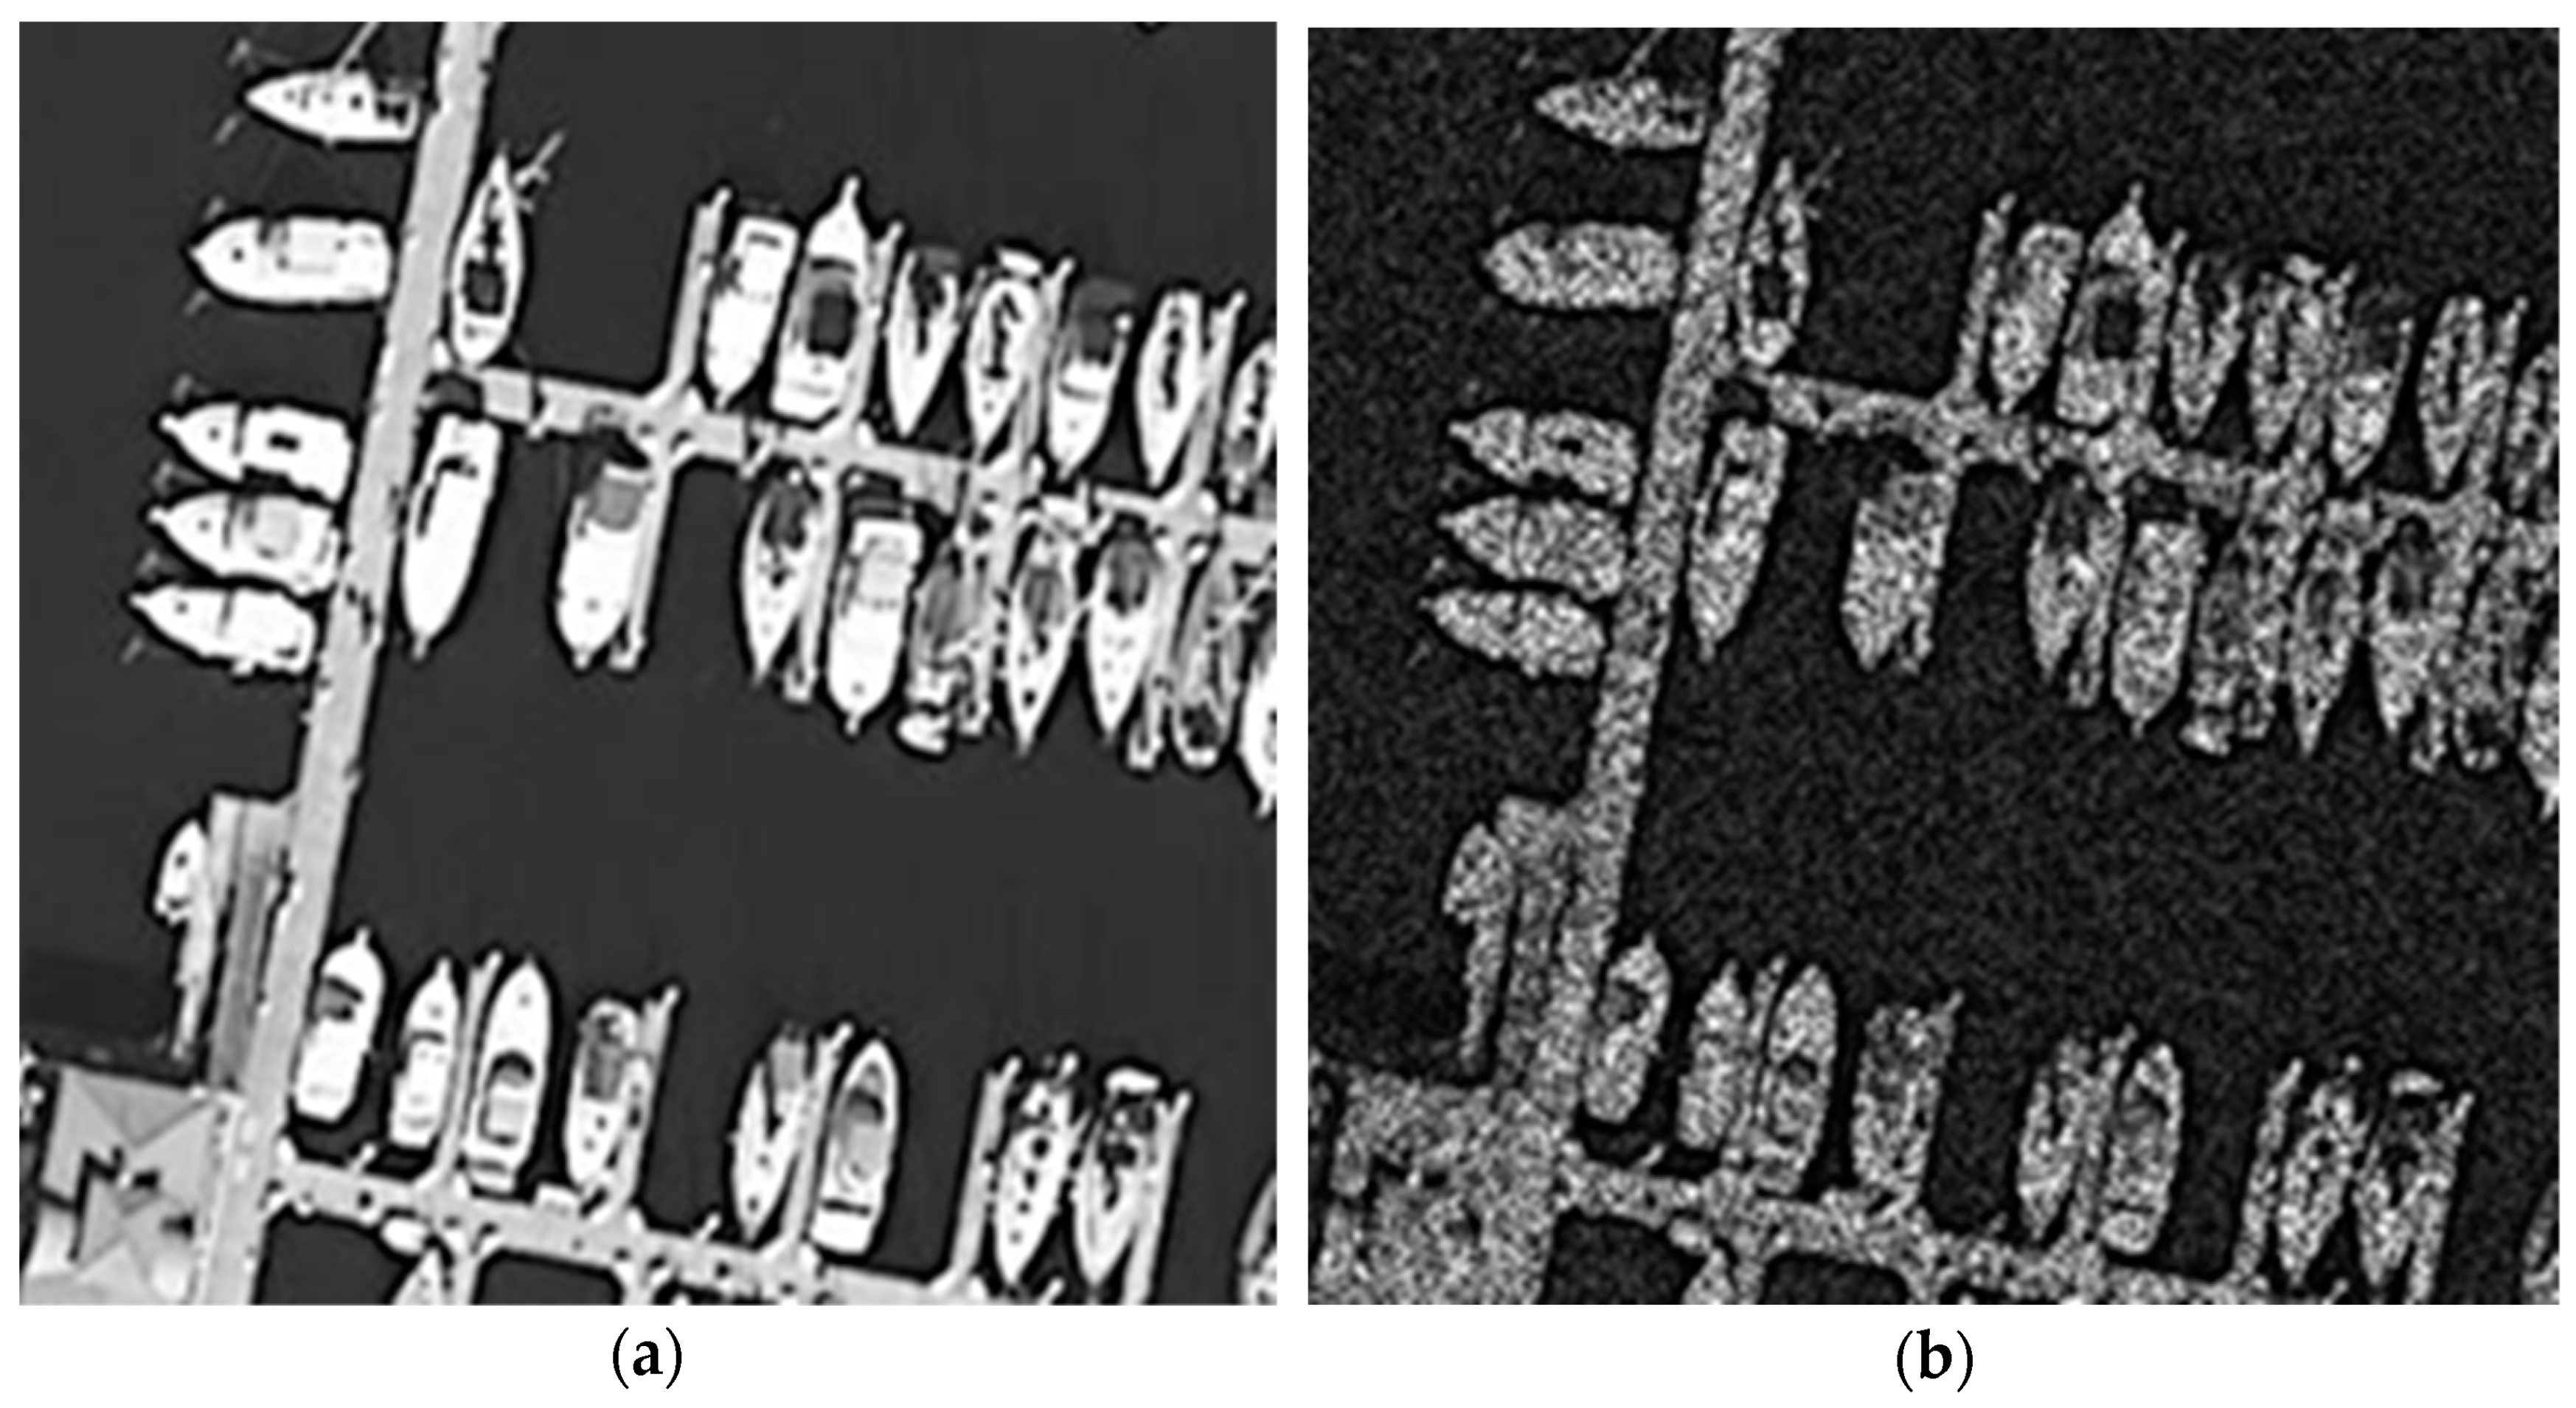
\includegraphics[width=0.5\linewidth]{../research-resources/SAR/sar-speckle.png}
	 \caption{a. Optical Image; b. SAR Image with speckle noise}
	\end{minipage}
 \end{figure}


 \indent Given that ice thickness is not a property directly measured by LiDAR nor captured in SAR imagery, sets of assumptions need to be made to deduce the property through related measurements. A leading paradigm in modeling ice thickness is through the assumption of hydrostatic equilibrium \cite{ICESat-2-L4-Product} \cite{Hutchings_Heil_Lecomte_Stevens_Steer_Lieser_2015} \cite{Forsström_Gerland_Pedersen_2011}, in which the properties of the ice sheet are deduced based upon the fact that the ice is buoyant in sea water (Figure 1.3). In this assumption, LiDAR measurements retrieve the elevations of the snow covered ice-surface in relation to the sea surface, and statistically infer the sea ice surface height. It's possible to relate the ice's total thickness to these elevation measurements by combining these relative heights with their associated substance densities (Equation 1.1). NASA's IS-2 L4 Along-Track Sea Ice Thickness product is a closely related example of this topic, and produced arctic ice thickness results between October 2018 and May 2022 \cite{ICESat-2-L4-Product}.
 \begin{figure}[htb]
	\centering
	\subfigure{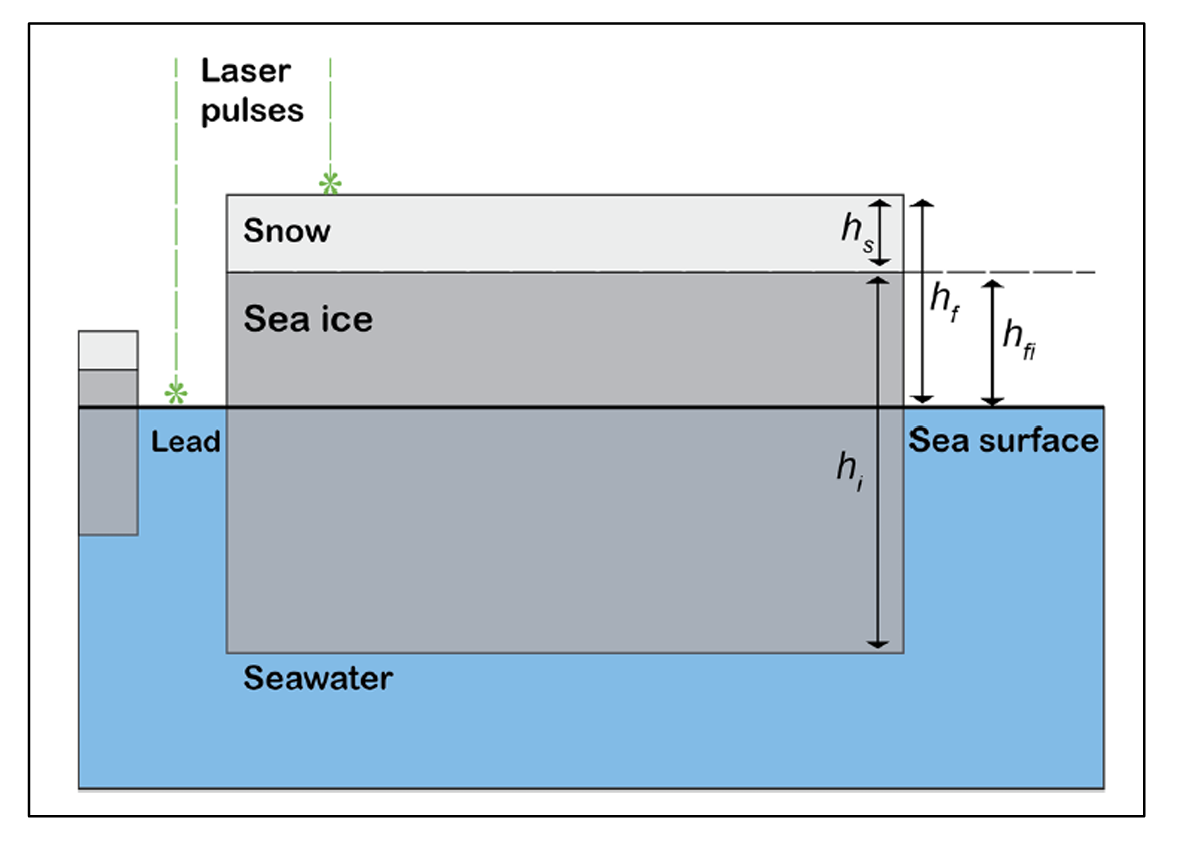
\includegraphics[width=.8\textwidth]{../research-resources/ice-sat-2/hydro-static-equillibrium.png}} 
	\caption{Ice Thickness Isostatic Assumption} \cite{ICESat-2-L4-Product}
	\label{fig:hydro-static-diagram}
\end{figure}

There are critiques with the established hydrostatic model. Ice density at a local scale is a variable property - it's dependent on factors like salinity, temperature, air volume and exposure \cite{sea-ice-properties}, and has a large enough observable difference that ice can be reliably classified into first and multi-year ice by SAR imaging alone \cite{SAR-U-Net}. Some studies delineate ice density by whether it's above or below the waterline, but find that air-rich above water ice only contributes to 10\% of the total density of the ice sheet. Given the variability, the exact local density of sea ice in the remote arctic is ephemeral, but generally agreed upon to be between 900-940 kg/m\^3, with some studies proposing a slightly wider range of 892-945 \cite{sea-ice-properties}. IS-2's L4 product settled to use a value of 916 kg/m\^3 for ice above and below the waterline.

\begin{equation}
	\label{eq:isostatic-equilibrium}
	\displaystyle h_i=\frac{\displaystyle h_f\rho_w}{(\rho_w-\rho_i)}+\frac{\displaystyle h_s(\rho_s-\rho_w)}{(\rho_w-\rho_i)}
\end{equation}
where:
\begin{conditions}
 \displaystyle h_i    &  Sea ice thickness \\   %	It'd be perfect to place the diagram of the sheet in the white space generated here in latex
 \displaystyle h_f    &  Freeboard height \\   %	It'd be perfect to place the diagram of the sheet in the white space generated here in latex
 \displaystyle h_s     &  Snow depth (m) \\      %	It'd be perfect to place the diagram of the sheet in the white space generated here in latex
 \rho_w 							&  Density of water \\   %	It'd be perfect to place the diagram of the sheet in the white space generated here in latex
 \rho_i 							&  Density of sea ice (900-940 kg/m\^3) \\   %	It'd be perfect to place the diagram of the sheet in the white space generated here in latex
 \rho_s 							&  Density of snow \\   %	It'd be perfect to place the diagram of the sheet in the white space generated here in latex
\end{conditions}

Even with established models in place to infer sea ice thickness from remote sensing methods, there is an innate problem with corroboration of these data sources. IS-2 has an orbit cycle of 91 days, meaning each location is surveyed only once nearly every 3 months \cite{ICESat-2-ATL10-Product}.

Discuss the prevalent sources of data as it stands - NSIDC as a data repository, NASA's Sentinel(1/2), IceSat-2, CryoSat satellites as periodic sources of data. Also give an overview as to how each medium works. This might need to span multiple paragraphs.

Importantly, it's important to recognize that laser altimetry is purely restricted to measuring Earth's surface - meaning the returned measurements are innately incapable of measuring sea-ice thickness, especially in the presence of snow on the surface. (Add source and put it in bibliography)

-Acknowledge that even with the best of the remote sensing methods, many extrapolations of ice-thickness rely on the same fundamental assumption (cite the source that mentioned this)-
Discuss isostatic equilibrium and how the physics of it requires density constants which aren't known or measured, and that density itself is dependent on factors like salinity, temperature, and age, all of which are unknown at local temporal and geographic scale. Current research attempts to quantify density have yielded a somewhat consistent range of values between **foo** and **bar**, but even this range has been disputed to be inaccurate [citing the IceSat-2 \& CryoSat study, the In-Situ analysis]. (Consider attaching the limitation of distance to the reference surface here, or include it in the limitations).

-Given the limitations, transition into the main idea of the thesis. Mapping LiDAR onto SAR?- 

Transition into how SAR imaging can capture a return that indicates sea ice thickness, but it's low resolution from Sentinel-2 prevents it from being local in context. The intuition behind the remainder of the thesis is to coincide precise IceSat-2 LiDAR and data derivatives with widespread SAR imaging, to determine whether sea-ice thickness can be a learnable property from SAR image returns.

The problems with this include the availability of applicable data (such as high-resolution SAR, as the precision of IceSat-2 is immediately lost with low-resolution imagery) and also the coincidence of these two modalities, both spatially and temporally.

-Remove everything from preliminary research - it's not important to the paper. Include the figures of all In-Situ measurements in the Beaufort Sea Region for demonstration of its unavailability especially in relation to the time horizon. Also include the buoyancy chart when discussing the limitations.-
% \indent After reviewing the preliminary research, this paper will move forward to a more targeted effort in obtaining and analyzing data to develop a machine learning model that can be used to predict ice thickness from said remote sensing methods. Chapter 2 will describe the process of obtaining the selected data, and Chapter 3 will discuss the methodology of developing the model.
\par



NASA's ICESat-2 L4 Along-Track Sea Ice Thickness highlights this problem, and addresses it using the assumption of hydro-static equilibrium. This equation, expressed as follows, uses the densities of water, sea-ice and snow, alongside the height of the snow to calculate the correlated thickness of the sea ice.


% Data of interest were the IceSat-2 ATL10 product and the NSIDC In-situ Dataset, selected for their combination of breadth and accuracy. Furthermore, the European Space Agency's requirements for sponsored data need to be explored to pursue the higher resolution SAR imagery hoped for. The in-situ measurements will provide an invaluable source of ground truth while the ATL10 product will drastically expand the flexibility and accessibility of sea ice freeboard data moving forward.

\paragraph*{}
The "On-Ice Arctic Sea Ice Thickness Measurements by Auger, Core, and Electromagnetic Induction, from the Late 1800s Onward, Version 2" contains 69,750 rows of data, spanning 5 categorized regions; the Arctic Ocean, the Beaufort Sea, Greenland Coast, Prudhoe Bay, and Russian Coast. Filtering down to the Beaufort Sea region, a region of interest, yields 23 separate studies ranging between 1958 and 2016.
\par
%%% Modify which figures you're showing and in what order. It's not apparent what direction you're trying to go from here if you leave all 3 together like this.


A single delivery of IceSat-2's ATL10 data product yields a '.h5' file, incompatible with traditional spreadsheets. To access IceSat-2 data in a meaningful way involved developing a script to extract relevant information according to the types enumerated in the data product specification. Columns of interest include the latitude, longitude, time, and calculated freeboard height for each of the three beam pairs.
// Consider adding perl and dynamically adding sample rows from the extracted .h5 file. This will give the reader context as to what's being gathered /

